\documentclass[11pt]{scrartcl}   %[draft,a4paper] R�nder testen
\usepackage{difaber}

\begin{document}

\renewcommand{\titlesubject}{Documentation of the ProM plugin}
\renewcommand{\titlename}{Uma}
\renewcommand{\titlesubtitle}{an Unfolding-based Model Analyzer}
\renewcommand{\titleauthor}{Dirk Fahland}
\renewcommand{\titleurl}{http://www.processmining.org/}
\renewcommand{\titlepurpose}{%%%
\textsbc{Uma} implements techniques for analyzing and simplifying process
models in ProM. The techniques build on the theory of \textsbc{unfoldings of
process models} and \textsbc{McMillan prefixes} to analyze the behavior of
process models in a compact, symbolic representation.}

\makenicetitle


\tableofcontents

\section{Plugin: Analyze Model}

This plugin allows to analyze behavioral properties of Petri net models.
While it is easy to use, understanding the analysis results requires a little
bit of knowledge on Petri nets and their behavior.

The plugin is called \textsbc{Analyze Model Using Uma} and takes as input a
Petri net.

\subsection{Requirements on the input}

Each transition of the Petri net must have a pre-place (i.e., an arc from a
place to the transition), and a post-place (i.e., an arc from the transition
to a place). The plugin will not run if the model does not satisfy this
requirement.

\subsection{Running the plugin} Select a Petri net and the plugin \textsbc{Analyze
Model Using Uma} from the plugin list. The plugin has several options as
shown in Figure~\ref{fig:analyze:step2}.

\begin{figure}[!htb]\centering
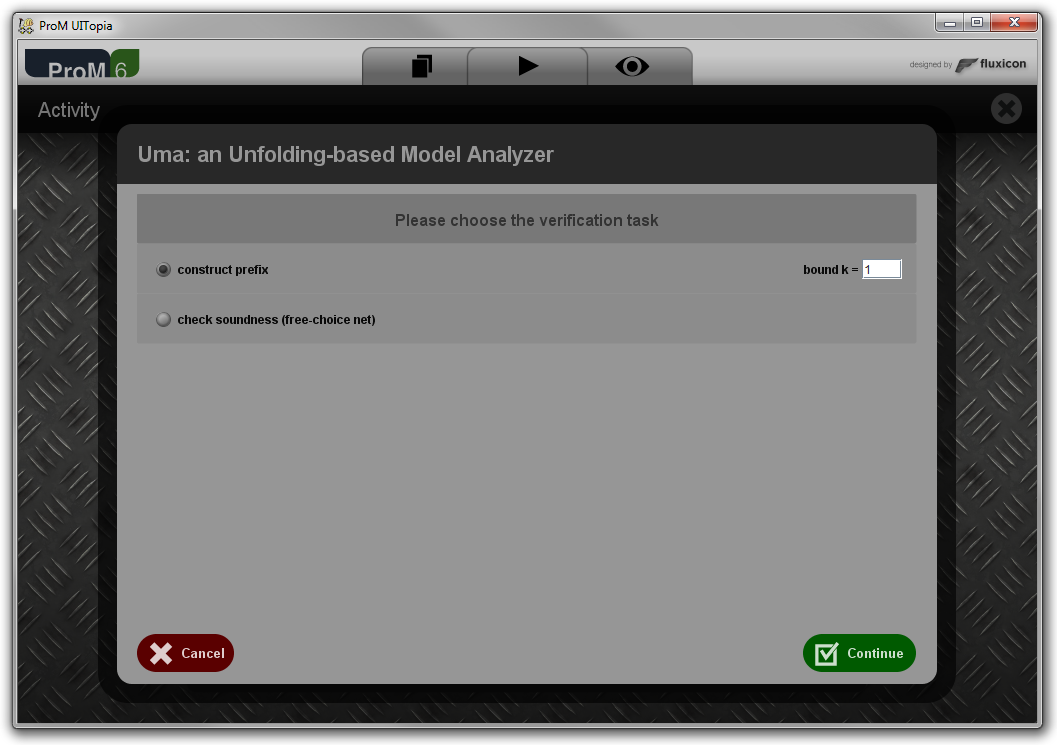
\includegraphics[width=.8\linewidth]{figs/analyze_02_options.png}
\caption{\textsbc{Analyze Model Using Uma}: Plugin options.}\label{fig:analyze:step2}
\end{figure}

\paragraph{construct prefix.} Constructs the so called McMillan
prefix of the Petri net, a tree-like structure representing the entire
behavior of the net in a compact form (similar to a state space) while
representing concurrency explicitly rather than by interleaving. The computed
prefix is returned as a result and can be inspected as shown in
Figure~\ref{fig:analyze:unfolding}. It allows a system modeler particulary to
understand which behavior can occur according to the model, for instance
which transitions can occur.

\begin{figure}[!htb]\centering
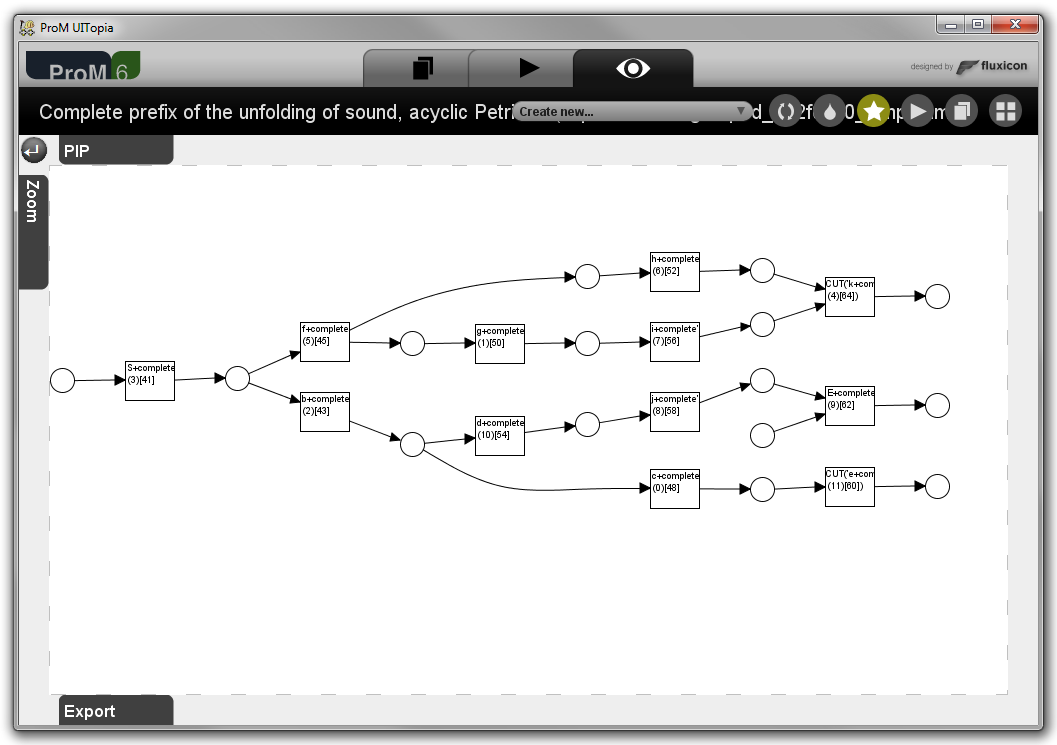
\includegraphics[width=.8\linewidth]{figs/analyze_03_result_unf.png}
\caption{Unfolding of a process model.}\label{fig:analyze:unfolding}
\end{figure}

The \textsbc{parameter $k$} is used to ensure termination of the plugin in
case the Petri net is unbounded. The plugin will stop when reaching a marking
where a place contains more than $k$ tokens. Default is $k = 1$.

\paragraph{check soundness.} Checks sounds of a free-choice Petri net. If the
net is sound, a corresponding result is shown. If the net is unsound, a
counter-example is returned showing the behavior that leads to a violation of
soundness which is in a free-choice net either a deadlock or an unsafe
marking. Figure~\ref{fig:analyze:unsound} shows such a counter example. It
currently needs expert knowledge to interpret the counter example and
identify the problem.

\begin{figure}[!htb]\centering
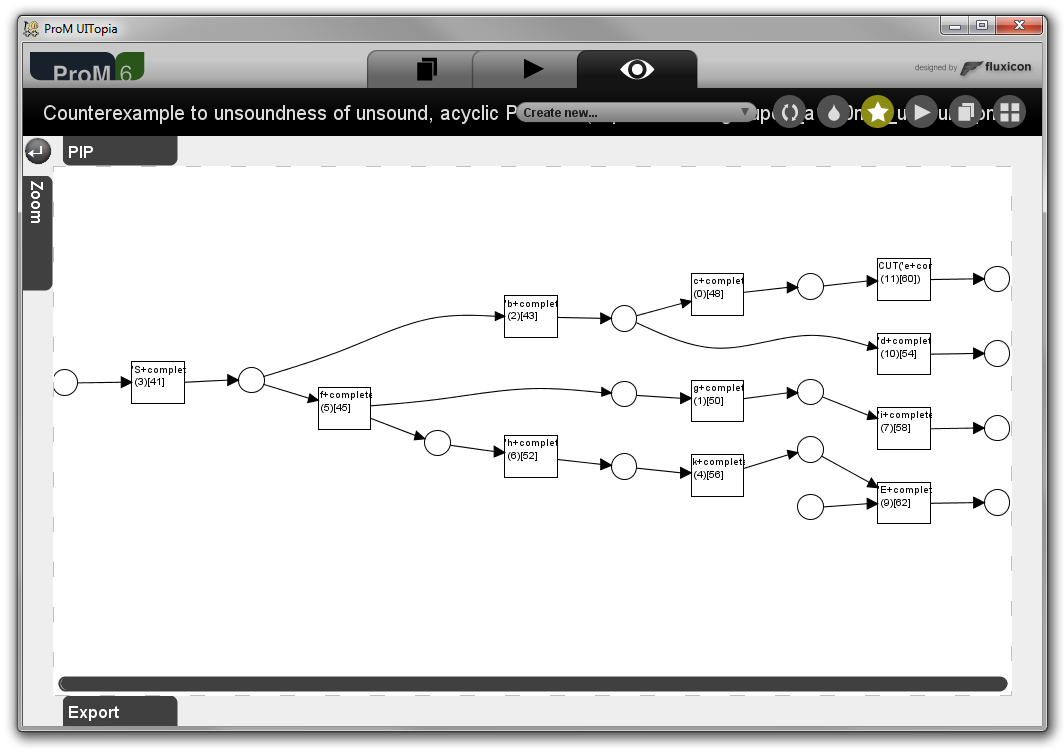
\includegraphics[width=.8\linewidth]{figs/analyze_04_result_unsound.png}
\caption{Counter-example showing unsoundness of a process model.}\label{fig:analyze:unsound}
\end{figure}


\section{Plugin: Simplify Mined Model}

This plugin allows to structurally simplify a process obtained from a process
mining algorithm while preserving that the model can replay the entire log.
The standard situation where this plugin may prove useful is when the model
that was discovered from a given log shows complex control-flow structures as
illustrated in Figure~\ref{fig:simplify:input}. The plugin to simplify such
models works on Petri net models and requires \emph{no expert knowledge} to
be used.

\begin{figure}[!htb]\centering
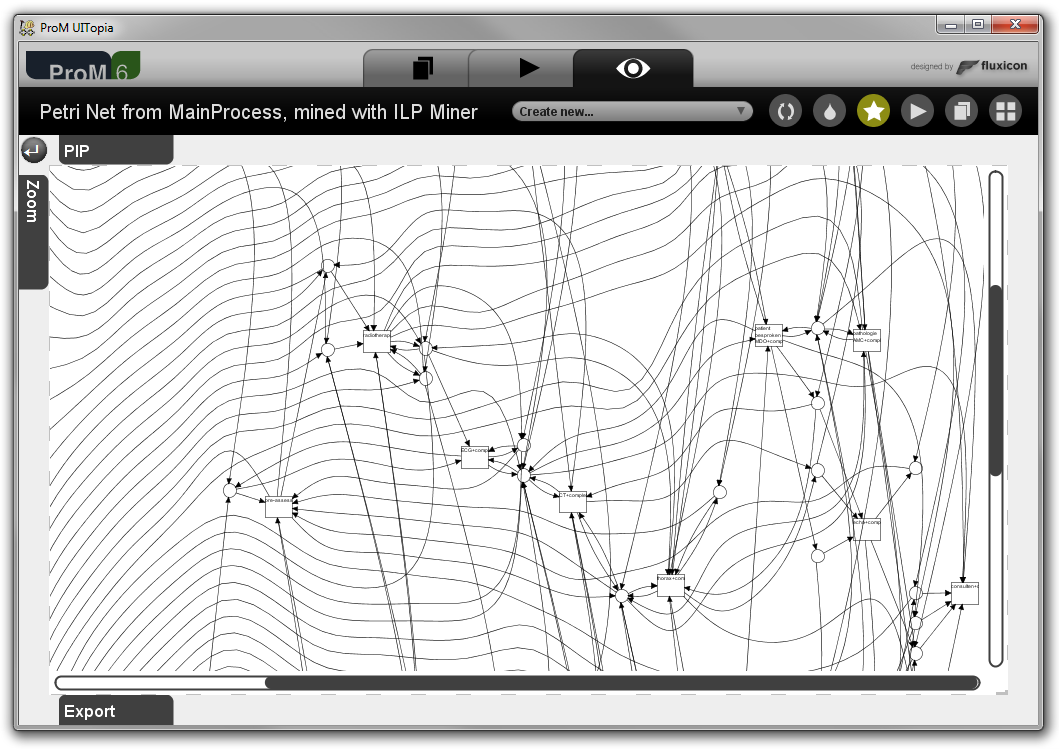
\includegraphics[width=.8\linewidth]{figs/simplify_01_original_model.png}
\caption{\textsbc{Simplify Mined Model}: typical mined process model with complex control flow structures.}\label{fig:simplify:input}
\end{figure}

The plugin is called \textsbc{Simplify Mined Model Using Uma} and takes as
input a log and a Petri net that was discovered from this log.

\subsection{Requirements on the input}

The plugin assumes that the Petri net was discovered from the provided log
and that the Petri net can replay the entire log, i.e., that the model has
fitness 1. Such models are obtained for instance using the \textsbc{ILP
Miner} or the \textsbc{Transition System Miner}.

In case the Petri net cannot replay the entire log, the simplified model
returned by the plugin will also cover only the behavior that could be
replayed on the Petri net. In the worst case, the returned net may be empty.

The plugin assumes that the Petri net has no arc weights or multiple arcs. In
case of arc weights or multiple arcs, the returned results are unpredictable.

\subsection{Running the plugin}

Select a Petri net and the log from which the Petri net was discovered and
and the plugin \textsbc{Simplify Mined Model Using Uma} from the plugin list.
The plugin implements a series of processing steps to simplify the given
model. Each step provides a different kind of simplification. You may choose
which simplification steps are run by the plugin using the configuration
panel shown in Figure~\ref{fig:simplify:options}.

\begin{figure}[!htb]\centering
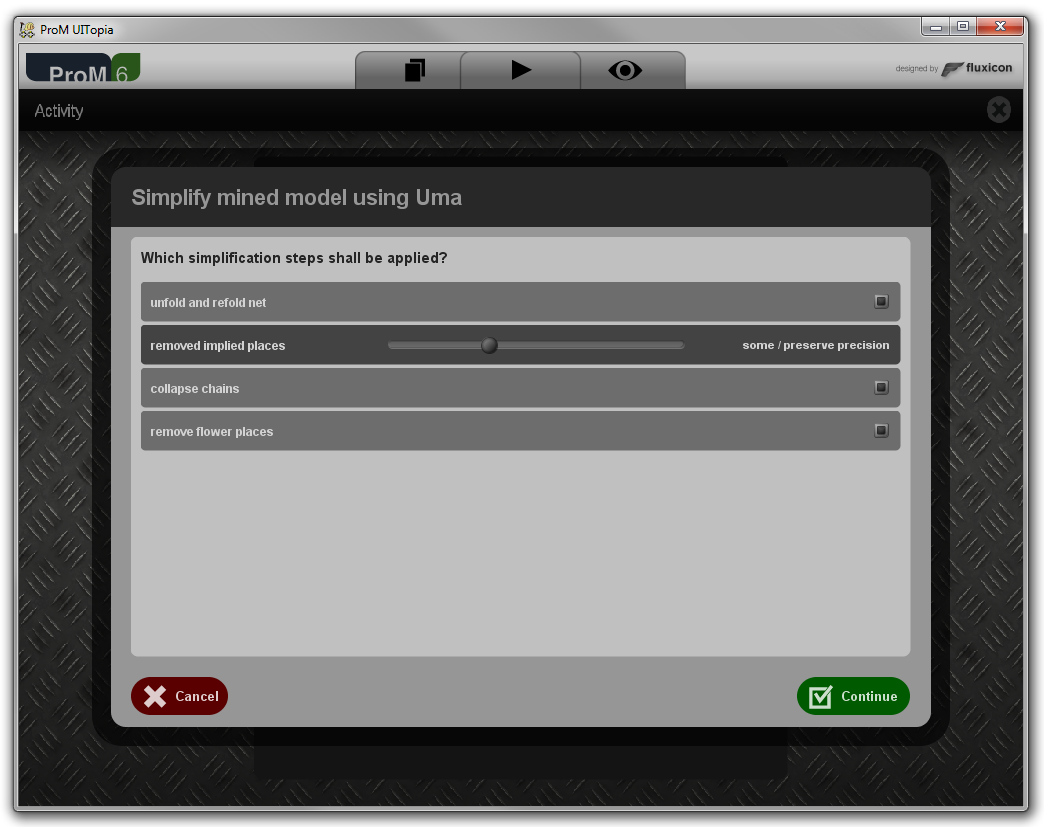
\includegraphics[width=.8\linewidth]{figs/simplify_02_options.png}
\caption{\textsbc{Simplify Mined Model}: plugin options.}\label{fig:simplify:options}
\end{figure}

\begin{description}
\item[\textsbc{unfold and refold net}] Unfold the process model the
    unfolding (similar to an execution tree) that represents exactly the
    behavior described in the log (up to different interleaving of
    concurrent transitions), and then refold the unfolded model. This
    step slightly simplifies the model and reduces generalization
    introduced by the mining algorithm.

\item[\textsbc{remove implied places}] Remove places from the net which
    do not contribute to restrict occurrences of transitions, i.e., where
    the net without the place has the same behavior as the net with the
    place (regarding the behavior in the log). This step allows to
    significantly simplify the model. However, simplification has to be
    traded for \emph{precision}, that is, how much additional behavior
    the net will allow for compared to the log. This trade-off can be
    configured:
    \begin{itemize}
    \item \textsbc{off} No place is removed.
    \item \textsbc{some / preserve precision} Remove only places that
        are implied wrt. the complete behavior of the model. The
        resulting model may still be complex, but it is guaranteed to
        show the same runs as before.
    \item \textsbc{more / preserve log causality} Remove only places
        that are implied wrt. the behavior seen in the log. The
        resulting model is less complex and it still exhibits the
        causal relations identified from the log.
    \item \textsbc{most / preserve connectivity} Remove all places
        that in some context represent an implied causal dependency,
        but ensure that the net remains connected. The resulting
        model is significantly simpler; however precision is lost to
        some degree. (default)
    \end{itemize}

\item[\textsbc{collapse chains}] Unfolding and refolding a net (first
    step) may introduce a chain of transitions labeled with the same
    action. This step collapses such chains into a loop, thus reducing
    the net's structure further while generalizing its behavior.

\item[\textsbc{remove flower places}] In some cases, the mining algorithm
    introduces \emph{flower places} from which many transitions consume
    tokens and immediately put the token back. Such places largely
    sequentialize the connected transitions while making the net
    structure very involved. In this step, flower places which are
    connected to more than 5\% of the net transitions are removed. This
    step may significantly simplify the net structure while generalizing
    the behavior.
\end{description}

All simplification steps are switched on by default. Upon clicking
\textsbc{continue}, the plugin will apply the chosen simplification steps and
return the simplified net. Figure~\ref{fig:simplify:output} shows the result
of applying all simplification steps on the model of
Figure~\ref{fig:simplify:input}.

\begin{figure}[!htb]\centering
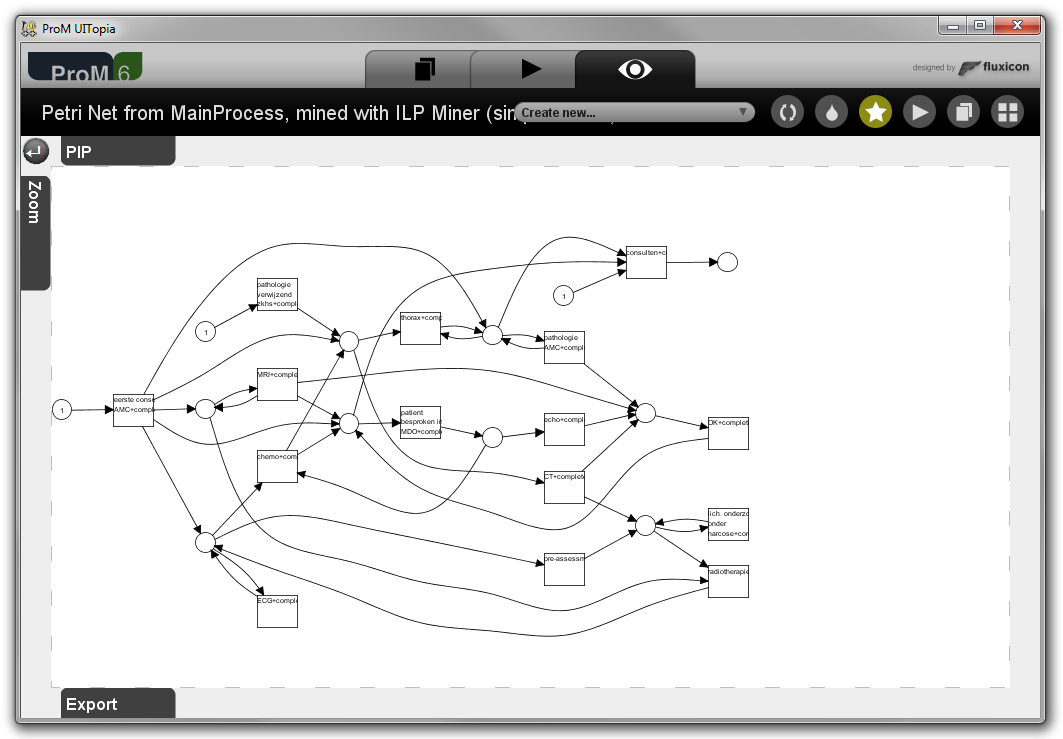
\includegraphics[width=.8\linewidth]{figs/simplify_03_result.png}
\caption{Model obtained by running the \textsbc{Simplify Mined Model} plugin on the model of Figure~\ref{fig:simplify:input}.}\label{fig:simplify:output}
\end{figure}

\section{Plugin: Repair Model}

The \textsbc{Repair Model} plugins allow to repair a given handmade process
model (given as a Petri net) to reflect the reality of process executions
that were observed in a log. The plugin can be applied in cases where a
conformance check between model and log reveals misconformances as shown in
Fig.~\ref{fig:repair:input}.

\begin{figure}[!htb]\centering
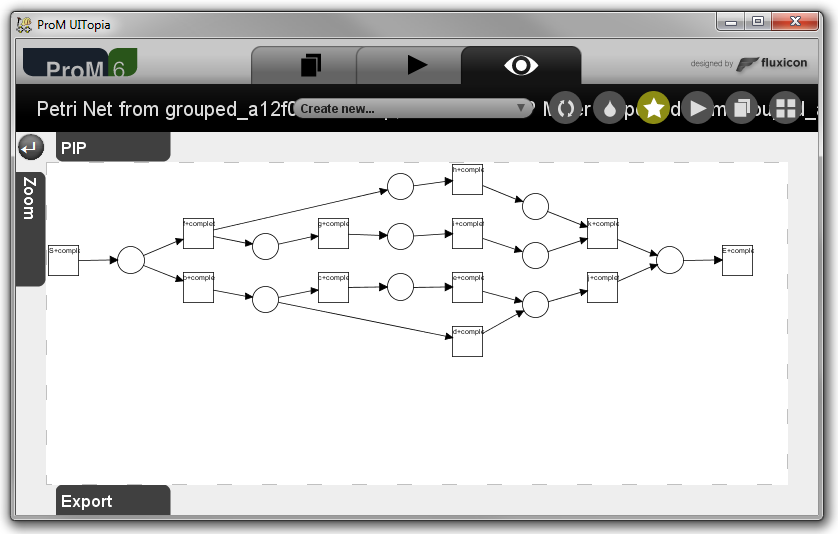
\includegraphics[width=.8\linewidth]{figs/repair_01a_model.png}
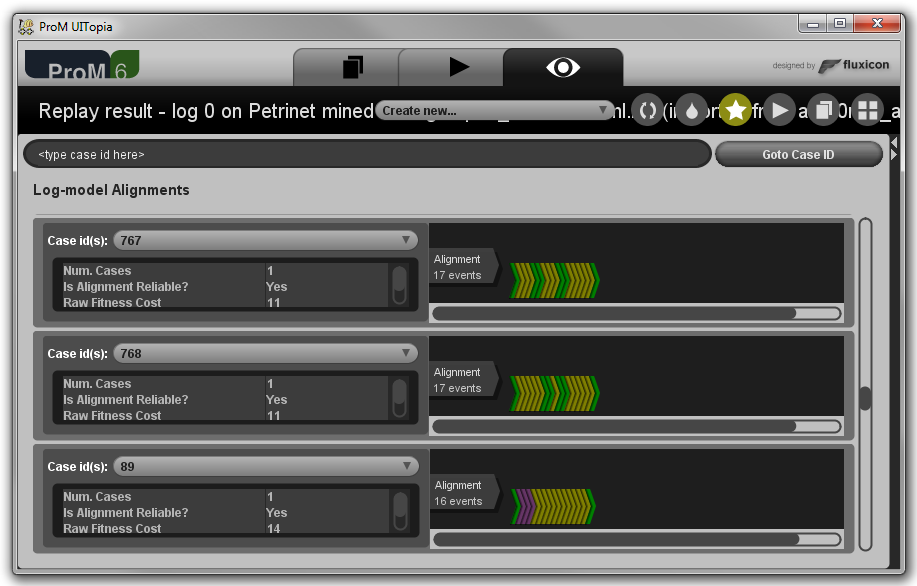
\includegraphics[width=.8\linewidth]{figs/repair_01b_misconformance.png}
\caption{\textsbc{Repair Model}: misconformances between log and model.}\label{fig:repair:input}
\end{figure}

\subsection{Requirements on the input}

The \textsbc{Repair Model} plugins require that the given model has a clear
notion of a final marking, that is, there is a particular marking that the
process has to reach. Moreover, the plugin will deliver best results if the
model is always able to reach the final marking. The \textsbc{Repair Model}
plugins will ask you to provide a final marking for your model if it is not
specified yet.

\subsection{Running the plugin}

Select a Petri net and the log describing executions of the process in
reality and run the plugin \textsbc{Repair Model} from the plugin list. The
plugin implements a series of processing steps to repair the given model.
Each step provides a different kind of repair. You may choose which repair
steps are run by the plugin using the configuration panel shown in
Figure~\ref{fig:repair:options}.

\begin{figure}[!htb]\centering
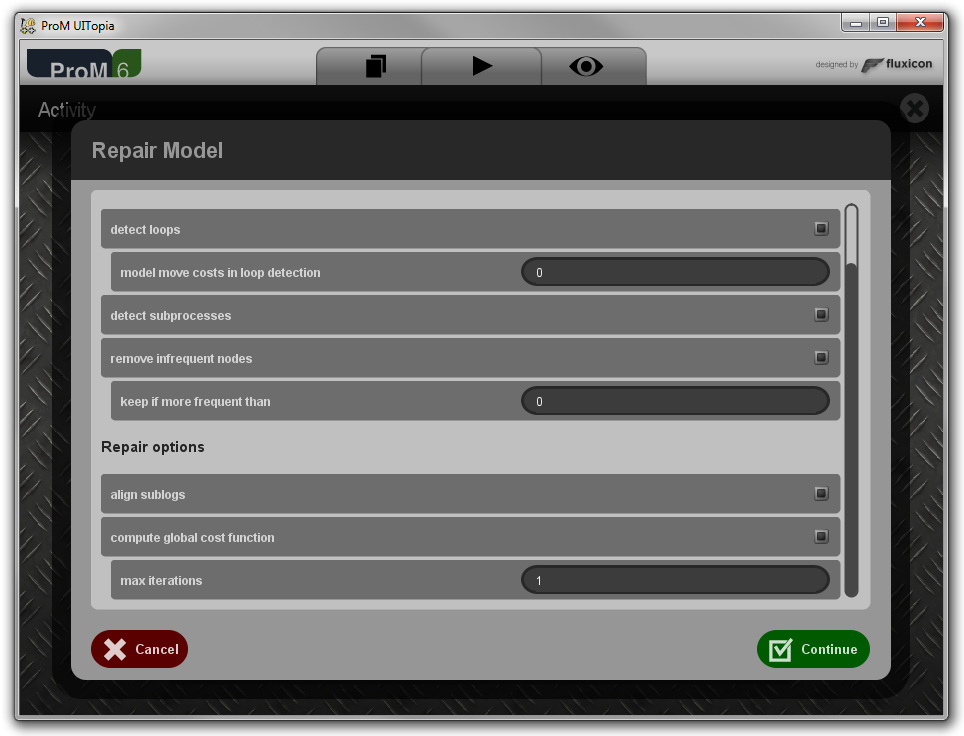
\includegraphics[width=.8\linewidth]{figs/repair_02_options.png}
\caption{\textsbc{Repair Model}: plugin options.}\label{fig:repair:options}
\end{figure}

The main model repair steps are the following:
%
\begin{description}
\item[\textsbc{detect loops}] Find parts of the process model that, when
    extended with a loop-back transition yield a structured loop that can
    replay traces of the log that could not be replayed on the original
    model. The option \textsbc{model move costs in loop detection} can be
    set to influence how loops are discovered. Generally, a value 0
    yields best results but may have a poor performance. A value >0 may
    yield faster results but give a worse quality in the repaired model.

\item[\textsbc{detect subprocesses}] For all remaining events that cannot
    be replayed on the original model, discover and add subprocesses that
    allow to replay these events.
\item[\textsbc{remove infrequent nodes}] Find parts of the process model
    that are not needed to replay the log, and remove them. Setting
    \textsbc{keep if more frequent than} to a value $> 0$ will also
    remove parts of the model that are used infrequently. This way, parts
    of the model that describe noisy behavior can be filtered out.
\end{description}
%
In addition, each repair step can be configured using 2 parameters:
%
\begin{description}
\item[\textsbc{align sublogs}] Decomposes and groups sequences of events
    that cannot be replayed into sets of very similar sequences. This
    typically yields more but smaller, and better structured,
    subprocesses.

\item[\textsbc{compute global cost function}] Misconformances between log
    and model are computed using a cost function. Enabling this option
    computes an improve cost function that yields better repairs (less
    changes to the model), at the price of additional computations.
    \textsbc{Max iterations} defines how often the current cost function
    shall be improved to, we found 1 iteration to be sufficient in most
    cases.
\end{description}
%
Once the parameters are set, \textsbc{ProM} will ask you to map transitions
of the model to event classes. Then the \textsbc{Repair Model} plugin will
run the specified model repair steps. Figure~\ref{fig:repair:repaired} shows
the model of Fig.~\ref{fig:repair:input} after repairs.
%
\begin{figure}[!htb]\centering
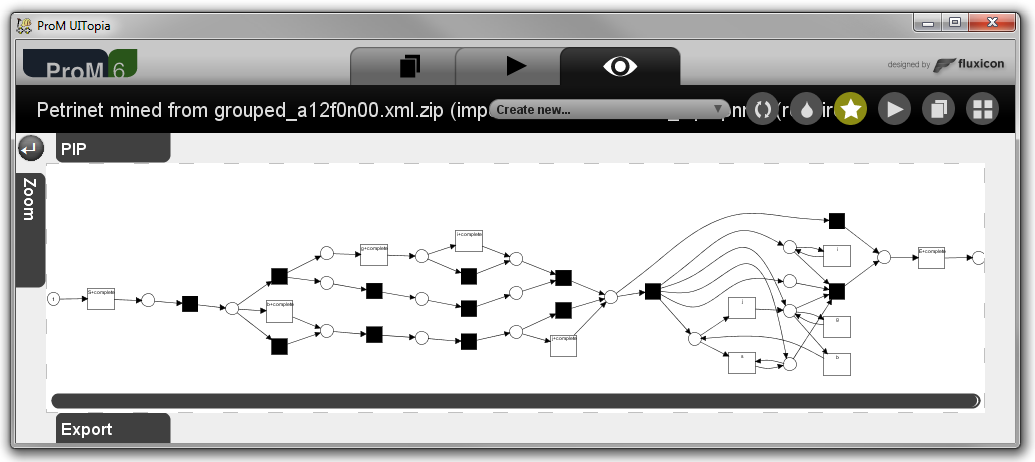
\includegraphics[width=.8\linewidth]{figs/repair_03_repaired.png}
\caption{\textsbc{Repair Model}: plugin options.}\label{fig:repair:repaired}
\end{figure}

The individual steps of the \textsbc{Repair Model} plugin can be controlled
in a more detailed way using the separate plugins for detecting loops,
detecting subprocesses, and removing infrequently used parts. Each of these
plugins takes as input model, log, and an \emph{alignment} between model and
log as it is returned by the conformance checker. The repair will always be
conducted with respect to the alignment, and choosing a particular cost
function, or a particular conformance checker, will yield a particular
alignment, and hence, a particular kind of repair. Two plugins for computing
alignments with global costs, and for computing alignments that improve the
discovery of loops are provided by \textsbc{Uma} as well.


\section{Technical Background and References}

Further information on the techniques implemented in \textsbc{Uma} can be
found in the following books and articles.

General information about the technique of unfoldings and McMillan prefixes
of Petri nets can be found in the following book:

\begin{itemize}
\item[] J. Esparza and K. Heljanko. \textsbc{Unfoldings - A Partial-Order
    Approach to Model Checking.} Springer-Verlag, 2008.
\end{itemize}

The technique for simplifying mined process models is described in the
following article:

\begin{itemize}
\item[] Dirk Fahland and Wil M.P. van der Aalst. \textsbc{Simplifying
    Mined Process Models: An Approach Based on Unfoldings.} In
    Proceedings of the 9th International Conference on Business Process
    Management, BPM 2011, volume 6896 of Lecture Notes in Computer
    Science, pages 362�378. Springer-Verlag, 2011
\end{itemize}

The technique for repairing process models is described in the following
article:

\begin{itemize}
\item[] Dirk Fahland and Wil M.P. van der Aalst. \textsbc{Repairing
    process models to reflect reality.} In Business Process Management
    2012, volume 7481 of Lecture Notes in Computer Science, pages
    229�245. Springer, 2012.
\end{itemize}

The source code of this plugin is available from the ProM website
\url{http://www.processmining.org/} under the GNU Affero General Public
License Version 3 or later.

\end{document}
